%%%%%%%%%%%%%%%%%%%%%%%%%%%%%%%%%%%%%%%%%%%%%%%%%%%%%%%%%%%%%%%%%
% Qualificacao de Doutorado / Dept Fisica, CFM, UFSC            %
% Eduardo@UFSC - 2015                                           %
%%%%%%%%%%%%%%%%%%%%%%%%%%%%%%%%%%%%%%%%%%%%%%%%%%%%%%%%%%%%%%%%%


%:::::::::::::::::::::::::::::::::::::::::::::::::::::::::::::::%
%                                                               %
%                   Anexo 1 -                                   %
%                                                               %
%***************************************************************%

\chapter{Artigos publicados}

\section{Diffuse ionized gas in galaxies across the Hubble sequence at the CALIFA resolution}
\label{apendice:DIGpaper0}

Artigo por \cite{Lacerda.etal.2018} (\texttt{10.1093/mnras/stx3022}).
Também disponível em {\em pre-print} (\texttt{arXiv:1711.07844}).

\cleardoublepage

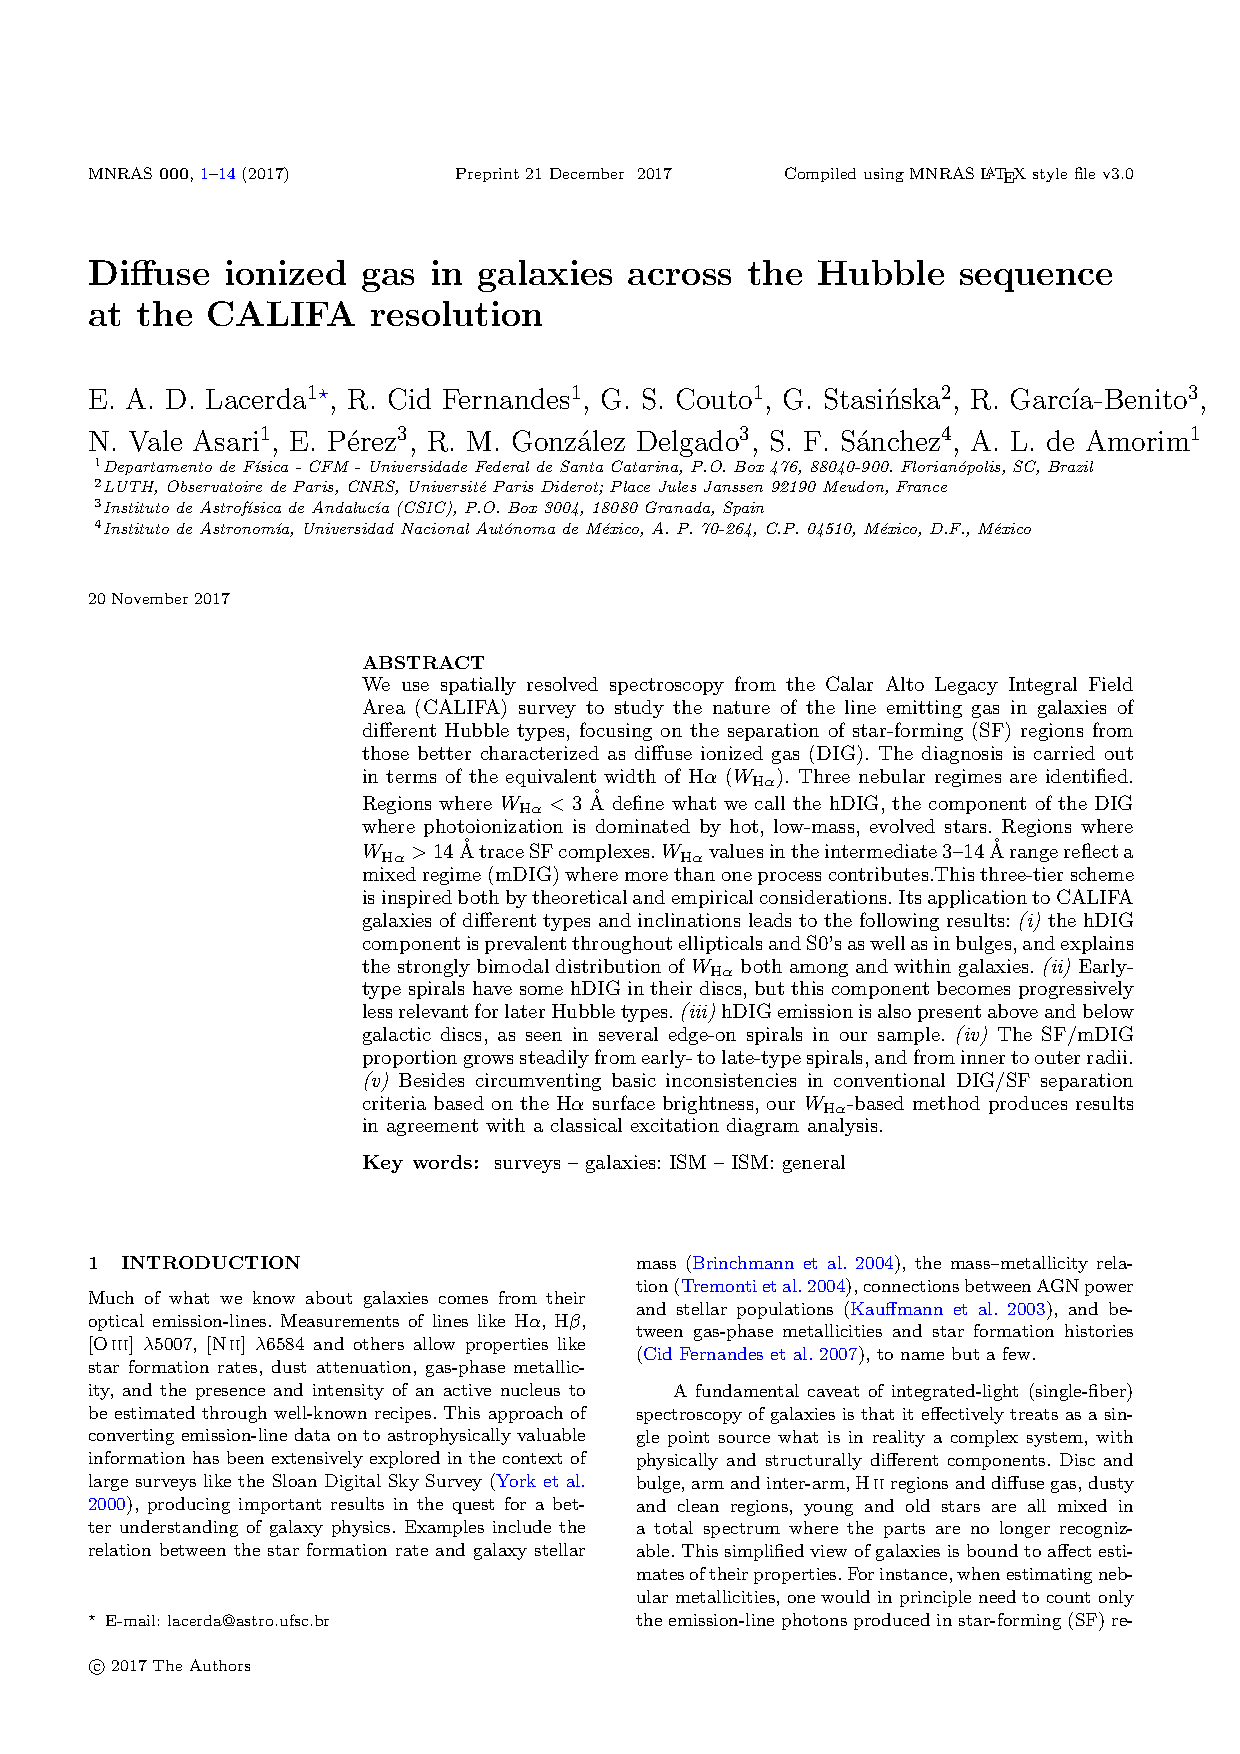
\includepdf[pages={-}]{artigos/DIGpaper0.pdf}

\section{CALIFA, the Calar Alto Legacy Integral Field Area survey. IV. Third public data release}
\label{apendice:SFSanchezDR3}

Artigo por \cite{SFSanchez.DR3.2016} (\texttt{doi:10.1051/0004-6361/201628661}).
Também disponível em {\em pre-print} (\texttt{arXiv:1604.02289}).

\cleardoublepage

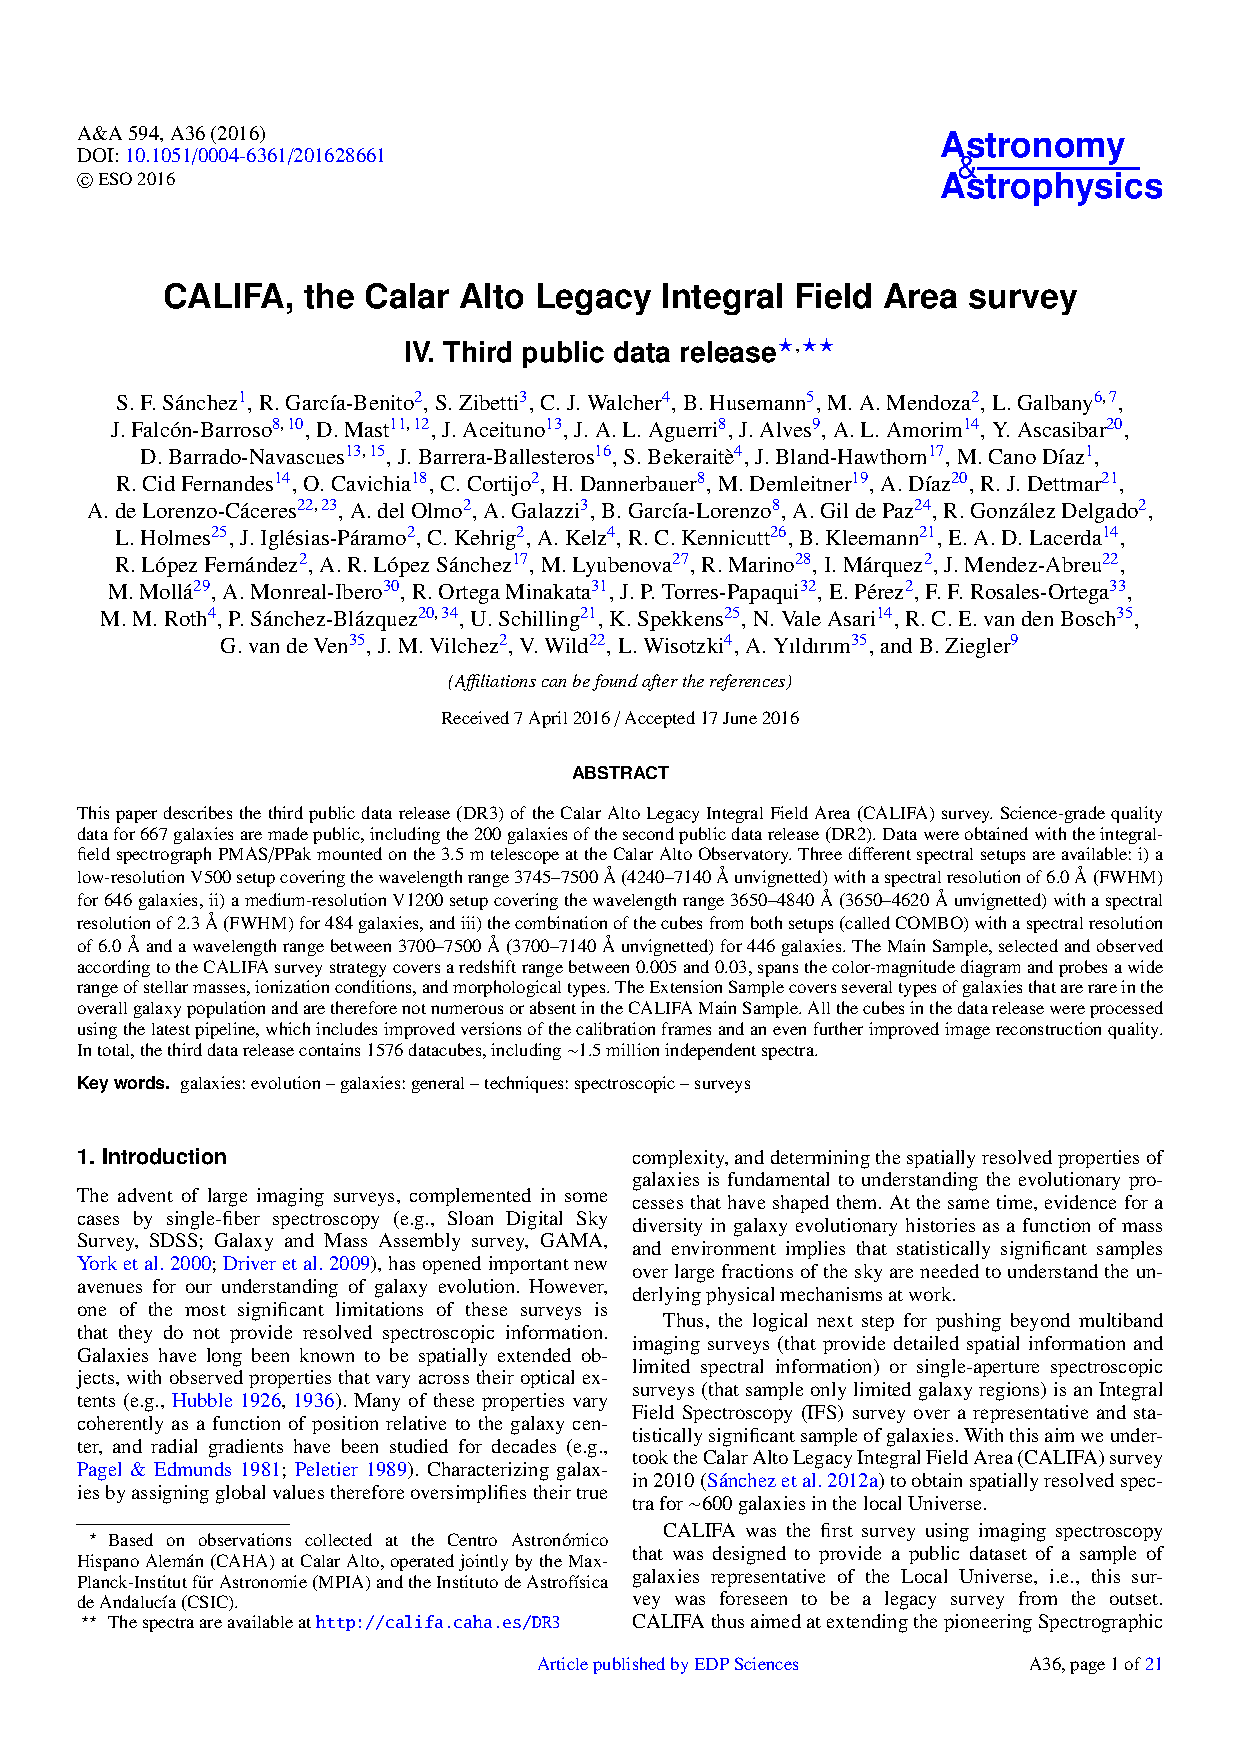
\includepdf[pages={-}]{artigos/DR3CALIFA-SFS2016.pdf}

% \section{CALIFA, the Calar Alto Legacy Integral Field Area survey. III. Second public data release}
% \label{apendice:GBetal2015a}
%
% Artigo por \cite{GarciaBenito.etal.2015a} (\texttt{doi:10.1051/0004-6361/201425080}).
% Também disponível em {\em pre-print} (\texttt{arXiv:1409.8302}).
%
% \cleardoublepage
%
% \includepdf[pages={-}]{artigos/GBetal2015a.pdf}
%
% \section{Insights on the stellar mass-metallicity relation from the CALIFA Survey}
% \label{apendice:GDetal2014b}
%
% Artigo por \cite{GonzalezDelgado.etal.2014b} (\texttt{doi:10.1088/2041-8205/791/1/L16}).
% Também disponível em {\em pre-print} (\texttt{arXiv:1407.1315}).
%
% \cleardoublepage
%
% 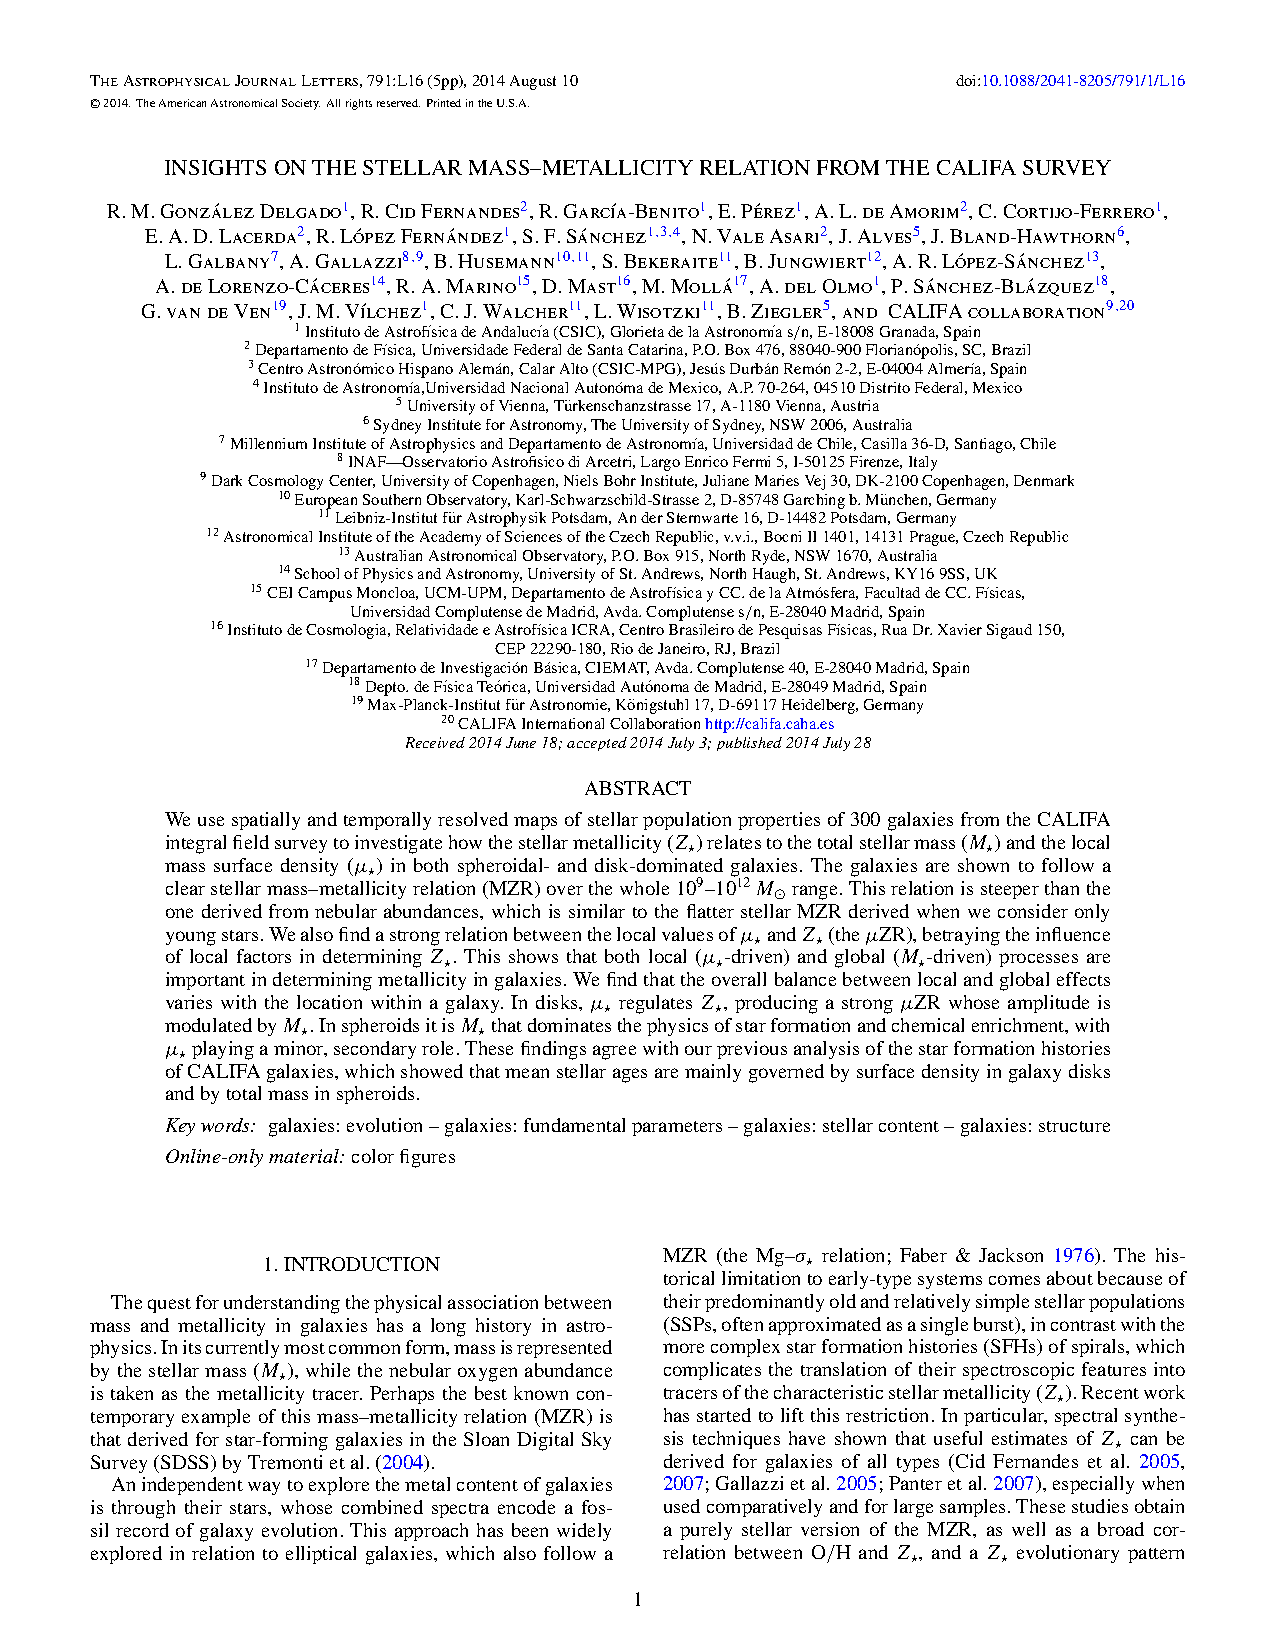
\includepdf[pages={-}]{artigos/GDetal2014b.pdf}
%
% \section{The CALIFA survey across the Hubble sequence. Spatially resolved stellar population properties in galaxies}
% \label{apendice:GDetal2015a}
%
% Artigo por \cite{GonzalezDelgado.etal.2015a} (\texttt{doi:10.1051/0004-6361/201525938}).
% Também disponível em {\em pre-print} (\texttt{arXiv:1506.04157}).
%
% \cleardoublepage
%
% \includepdf[pages={-}]{artigos/GDetal2015a.pdf}

% End of this chapter
